\documentclass{article}

\usepackage{amssymb}
\usepackage{graphicx}
\usepackage[colorlinks,linkcolor=blue]{hyperref}

\begin{document}
    \title{\textbf{TransportIDE} -- An integrated transportation system design and test environment}
    \author{Georg Hackenberg}
    \maketitle
    
    \begin{abstract}
        Due to many reasons transportation systems have to become more and more efficient.
        This observation holds true both for person transport and for good transport, on public infrastructure and on private infrastructure.
        Designing efficient transportation systems is a difficult undertaking due to the vast size of the solution space and the emergent dynamics of the system components.
        Transportation system designers need appropriate tools to explore the design space and test solutions quickly and reliably.
        In this paper, we propose a simulation-based environment for transportation system design and test, which is built on a solid system theory.
        Furthermore, we demonstrate possible applications such as comparison of different infrastructure and control algorithm designs.
    \end{abstract}
    
    \section{Introduction}
    \label{sec:intro}
    TODO~\cite{key}

    \subsection*{Research question}
    How can we support the design and test of transportation infrastructures and control algorithms better?
    Which modeling and simulation technique represents an appropriate abstraction for the domain?
    Which software architecture is appropriate for an integrated design and test environment?
    Which application scenarios should be supported on top of this environment?

    \subsection*{Research methodology}
    To answer the above questions, we apply and combine two research methodologies.
    First we conduct a literature review to understand the state of the art in transportation system design and test.
    Second we use iterative and incremental software development with regular feedback from stakeholders to develop our a new dedicated approach.

    \subsection*{Document outline}
    In the following, w e first present related work on transportation system design and test in Section~\ref{sec:related}.
    Then we describe the underlying system theory of our approach in Section~\ref{sec:theory}.
    Afterwards, we explain our software architecture in Section~\ref{sec:arch}.
    Thereafter, we demonstrate three software applications in Section~\ref{sec:app}.
    Finally, we draw our conclusion in Section~\ref{sec:con}.

    \section{Related work}
    \label{sec:related}
    TODO

    \section{System theory}
    \label{sec:theory}
    In the following, we explain the underlying system theory.
    In Section~\ref{sec:concepts} we introduce the concepts, which can be used for transportation system design.
    Then, in Section~\ref{sec:events} we describe the discrete event simulation semantics of transportation system designs.

    \subsection{Concepts}
    \label{sec:concepts}
    Figure~\ref{fig:concepts} provides an overview of the concepts included in our approach.
    We use intersections and segments for describing the transportation infrastructure.
    Then, we use locations and stations for describing the charging infrastructure.
    Furthermore, we use locations and vehicles for describing the transportation capacities and their initial state.
    Finally, we use location-times and demands for describing the transportation loads.

    \begin{figure}[htbp]
        \centering
        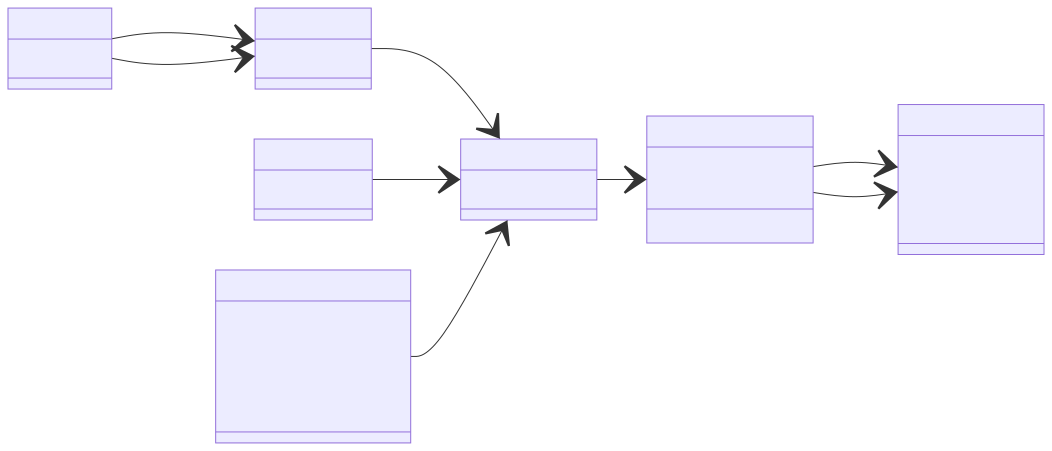
\includegraphics[width=\textwidth]{../../diagrams/model/classes-v0.png}
        \caption{Concepts in UML class diagram notation}
        \label{fig:concepts}
    \end{figure}

    In the following, we describe each concept in more detail including its attributes and relations.
    Also, we introduce a basic mathematical notation, which allows us to formulate the discrete event simulation semantics of transportation systems in the next section.

    \paragraph{Intersections}
    Intersections define the corner stones of the transportation infrastructure.
    Each intersection must have a coordinate in the corresponding reference coordinate system.
    Mathematically, intersections can be described as elements $i \in I$ with 
    \begin{itemize}
        \item coordinate property function $P_{I.C}: I \rightarrow \mathbb{R}^3$.
    \end{itemize}

    \paragraph{Segments}
    Segments define the connections between the intersections.
    Each segment must define a source intersection and a target intersection, which are connected by the segment.
    Furthermore, each segment must define a width and a maximum drive speed.
    Finally, the length of the segment can be computed from the coordinates of the source intersection and the target intersection.
    Mathematically, segments can be described as elements $(i_s, i_t) \in I \times I = Seg$ with source intersection $i_s$, target intersection $i_t$,
    \begin{itemize}
        \item width property function $P_{Seg.W}: Seg \rightarrow \mathbb{N}$,
        \item maximum drive speed property function $P_{Seg.MDS}: Seg \rightarrow \mathbb{R}^+$, and
        \item length property function $P_{Seg.L}: Seg \rightarrow \mathbb{R}_0^+$ such that $P_{Seg.L}(i_s, i_t) = |P_{I.C}(i_t) - P_{I.C}(i_s)|$, where $|\cdot|: \mathbb{R}^3 \times \mathbb{R}^3 \rightarrow \mathbb{R}_0^+$ represents a suitable distance function.
    \end{itemize}

    \paragraph{Locations (auxiliary)}
    Locations represent an auxiliary concept and define dedicated positions on the transportation infrastructure.
    Each location must define a corresponding segment and a travelled distance on that segment.
    Mathematically, locations can be described as elements $(seg, d) \in Seg \times \mathbb{R}_0^+ = L$ with segment $seg$ and distance $d$ such that $d \leq P_{Seg.L}(seg)$.

    \paragraph{Location-times (auxiliary)}
    Location-times also represent an auxiliary concept and define dedicated positions on the transportation infrastructure at particular time points.
    Each location-time must define a corresponding location and the desired time point.
    Mathematically, location-times can be described as elements $(l, t) \in L \times \mathbb{R}_0^+ = LT$ with location $l$ and time point $t$.

    \paragraph{Stations}
    Stations define the charging infrastructure for vehicles to refill their batteries.
    Each station must define a location on the transportation infrastructure and a maximum charge speed.
    Mathematically, stations can be described as elements $sta \in Sta$ with
    \begin{itemize}
        \item location property function $P_{Sta.L}: Sta \rightarrow L$ and
        \item maximum charge speed property function $P_{Sta.MCS}: Sta \rightarrow \mathbb{R}^+$.
    \end{itemize}

    \paragraph{Vehicles}
    Vehicles define the transportation capacities available on the transportation infrastructure.
    Each vehicle must define a battery capacity, a demand capacity, a maximum drive speed, and a maximum charge speed.
    Furthermore, each vehicle must define an initial location on the transportation infrastructure and an initial battery level.
    Mathematically, vehicles can be described as elements $v \in V$ with
    \begin{itemize}
        \item battery capacity property function $P_{V.BC}: V \rightarrow \mathbb{R}^+$,
        \item demand capacity property function $P_{V.DC}: V \rightarrow \mathbb{R}^+$,
        \item maximum drive speed property function $P_{V.MDS}: V \rightarrow \mathbb{R}^+$,
        \item maximum charge speed property function $P_{V.MCS}: V \rightarrow \mathbb{R}^+$,
        \item initial location property function $P_{V.IL}: V \rightarrow L$, and
        \item initial battery level property function $P_{V.IBL}: V \rightarrow \mathbb{R}_0^+$.
    \end{itemize}

    \paragraph{Demands}
    Demands define the transportation loads that temporarily consume the transportation capacities.
    Each demand must define a pick-up location and earliest pick-up time as well as a drop-off location and a latest drop-off time.
    Mathematically, demands can be described as elements $d \in D$ with
    \begin{itemize}
        \item pick-up property function $P_{D.PU}: D \rightarrow LT$ with $P_{D.PU}(d) = (l_d^{PU},t_d^{PU})$, and
        \item drop-off property function $P_{D.DO}: D \rightarrow LT$ with $P_{D.DO}(d) = (l_d^{DO},t_d^{DO})$ such that $l_d^{PU} \neq l_d^{DO}$ and $t_d^{PU} < t_d^{DO}$.
    \end{itemize}

    \subsection{Events}
    \label{sec:events}
    TODO

    \subsubsection{E1 -- Vehicle at intersection}
    TODO

    \subsubsection{E2 -- Faster vehicle at slower vehicle back}
    TODO

    \subsubsection{E3 -- Slower vehicle at faster vehicle back}
    TODO

    \subsubsection{E4 -- Vehicle at demand pick-up location}
    TODO

    \subsubsection{E5 -- Vehicle at demand drop-off location}
    TODO

    \subsubsection{E6 -- Vehicle at station}
    TODO

    \subsubsection{E7 -- Vehicle battery full}
    TODO

    \subsubsection{E8 -- Vehicle battery empty}
    TODO

    \section{Software architecture}
    \label{sec:arch}
    TODO Figure~\ref{fig:0}

    \begin{figure}[htbp]
        \centering
        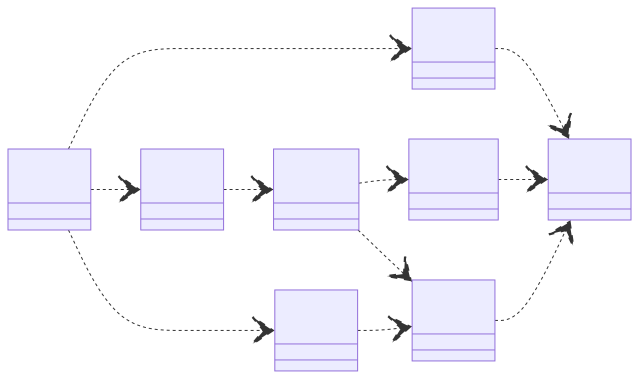
\includegraphics[width=0.7\textwidth]{../../diagrams/architecture.png}
        \caption{Module architecture}
        \label{fig:0}
    \end{figure}

    \subsection{Controller}
    \label{sec:controller}
    TODO Figure~\ref{fig:2}

    \begin{figure}[htbp]
        \centering
        \includegraphics[width=\textwidth]{../../diagrams/controller/classes.png}
        \caption{Controller interface}
        \label{fig:2}
    \end{figure}

    \subsubsection{Manual}
    TODO

    \subsubsection{Random}
    TODO
    
    \subsubsection{Greedy}
    TODO

    \subsubsection{Smart}
    TODO

    \subsubsection{Switchable}
    TODO

    \subsection{Statistics}
    \label{sec:statistics}
    TODO Figure~\ref{fig:3}

    \begin{figure}[htbp]
        \centering
        \includegraphics[width=0.5\textwidth]{../../diagrams/statistics/classes.png}
        \caption{Statistics interface}
        \label{fig:3}
    \end{figure}

    \section{Software application}
    \label{sec:app}
    TODO

    \subsection{Basic simulation}
    \label{sec:basic}
    TODO Figure~\ref{fig:4}

    \begin{figure}[htbp]
        \centering
        \includegraphics[width=\textwidth]{../../screenshots/basic-simulation.png}
        \caption{Basic simulation}
        \label{fig:4}
    \end{figure}

    \subsection{Controller comparison}
    \label{sec:controller-comparison}
    TODO Figure~\ref{fig:5}

    \begin{figure}[htbp]
        \centering
        \includegraphics[width=\textwidth]{../../screenshots/controller-comparison.png}
        \caption{Controller comparison}
        \label{fig:5}
    \end{figure}

    \subsection{Infrastructure comparison}
    \label{sec:infrastructure-comparison}
    TODO Figure~\ref{fig:6}

    \begin{figure}[htbp]
        \centering
        \includegraphics[width=\textwidth]{../../screenshots/infrastructure-comparison.png}
        \caption{Infrastructure comparison}
        \label{fig:6}
    \end{figure}

    \section{Conclusion}
    \label{sec:con}
    TODO

    \bibliographystyle{plain}
    \bibliography{main}
\end{document}